\documentclass[a1paper]{tikzposter}

\usepackage[utf8]{inputenc}
\usepackage[T1]{fontenc}
\usepackage[english]{babel}
\usepackage{amsmath,amssymb}
\usepackage[makeroom]{cancel}
\usepackage{multicol}
\usepackage{pgfplots}
\usepackage{pgfplotstable}
\usepackage{subcaption}
\usepackage{bm}
\usepackage{empheq}
\usepackage{multicol}
\usepackage{adjustbox} 
\usepackage[cm]{sfmath}
\usepackage{multirow}
\usepackage{gnuplottex}%[miktex]%[shell]
\usepackage{lipsum}
\usepackage{booktabs}
\usepackage{array}
\usepackage{float}
\usepackage{csquotes}
\usepackage{tcolorbox}
\usepackage[maxnames=1]{biblatex}
\usepackage{textcomp}


\AtNextBibliography{\scriptsize}
\addbibresource{Ref.bib}

\definecolor{myDarkRed}{RGB}{220,0,0}


\usepgfplotslibrary{fillbetween}
\usetikzlibrary{calc,arrows,patterns,plotmarks,shapes,er,3d,automata,backgrounds,topaths,trees,petri,mindmap}
\pgfplotsset{compat=1.16}



\usetikzlibrary{positioning}
\usepackage{pgf, tikz, pgfplots}
\usepackage{pgfplotstable}
\pgfplotsset{compat=1.16}

\definecolor{colorAir}{RGB}{2,121,178}
\definecolor{colorBlood}{RGB}{133,6,6}

\definecolor{colorA}{RGB}{49,140,231}   % Bleu Roi
\definecolor{colorB}{RGB}{238,16,16}    % Garance
\definecolor{colorC}{RGB}{34,120,15}    % Vert de vessie
\definecolor{colorD}{RGB}{136,77,167}   % Améthyste
\definecolor{colorE}{RGB}{158,14,64}    % Pourpre


\tikzposterlatexaffectionproofoff %shows small comment on how the poster was made at bottom of poster


% color to use
\definecolorpalette{bgColor} {
  \definecolor{colorOne}{rgb}{0.69, 0.93, 0.93}
  % \definecolor{colorOne}{rgb}{0.69, 0.93, 0.93}
  \definecolor{colorTwo}{rgb}{0.49, 0.01, 0.03}
%   \definecolor{colorTwo}{named}{brown}
  \definecolor{colorThree}{named}{blue}
  \definecolor{myblue}{RGB}{0,0,145}
}

% how to use color
\definecolorstyle{mystyle}{
    % color by default
  \definecolor{colorOne}{named}{gray}
  \definecolor{colorTwo}{named}{red}
  \definecolor{colorThree}{named}{blue}
}{
  \colorlet{backgroundcolor}{colorOne!50}       % background color
  \colorlet{framecolor}{black}                  % ???
  \colorlet{titlefgcolor}{myblue!80!black}    % ???
  \colorlet{titlebgcolor}{white}                % ???
  \colorlet{blocktitlebgcolor}{myblue}   % block-left-color
  \colorlet{blocktitlefgcolor}{white}       % block title color
  \colorlet{blockbodybgcolor}{white}         % block bg color
  \colorlet{blockbodyfgcolor}{black}        % block text color
  \colorlet{innerblocktitlebgcolor}{white}  % ???
  \colorlet{innerblocktitlefgcolor}{colorTwo}   % ???
  \colorlet{innerblockbodybgcolor}{white}       % ???
  \colorlet{innerblockbodyfgcolor}{black}       % ???
  \colorlet{notefgcolor}{black}
  \colorlet{notebgcolor}{colorTwo}
  \colorlet{noteframecolor}{colorTwo}
}

% title style
\definetitlestyle{mytitle}{
    width=0.9\paperwidth, roundedcorners=0, linewidth=0pt, innersep=1.5cm,
    titletotopverticalspace=0mm, titletoblockverticalspace=20mm,
    titlegraphictotitledistance=10pt, titletextscale=1
}{
   % \draw[draw=none, bottom color=framecolor, top color=titlebgcolor]%
   % (\titleposleft,\titleposbottom) rectangle (\titleposright,\titlepostop); %
}

% block style
\defineblockstyle{myblock}{
    titlewidthscale=1, bodywidthscale=1, titleleft,
    titleoffsetx=0pt, titleoffsety=0pt, bodyoffsetx=0pt, bodyoffsety=0pt,
    bodyverticalshift=0pt, roundedcorners=0, linewidth=0pt, titleinnersep=5mm, 
    bodyinnersep=4mm 
}{
    \ifBlockHasTitle%
        \draw[draw=none, left color=blocktitlebgcolor, right color=blocktitlebgcolor]
           (blocktitle.south west) rectangle (blocktitle.north east);
    \fi%
    \draw[draw=none, fill=blockbodybgcolor] %
        (blockbody.north west) [rounded corners=20] -- (blockbody.south west) --
        (blockbody.south east) [rounded corners=0]-- (blockbody.north east) -- cycle;
}

% theme set of styles
\definelayouttheme{mytheme}{
  \usecolorstyle[colorPalette=bgColor]{mystyle}
  \usebackgroundstyle{Rays}
  \usetitlestyle{mytitle}
  \useblockstyle{myblock}
  \useinnerblockstyle{Slide}
  \usenotestyle{Default}
}

\usetheme{mytheme}

\settitle{
  % \parbox{\linewidth}{\color{titlefgcolor} {\bfseries \Huge \@title}}
  \centering \vbox{
    \vspace{-1cm}
    \@titlegraphic \\[\TP@titlegraphictotitledistance]
    \vspace{-4cm}
    \centering
    % \vspace*{-12.5cm}
%     % \begin{minipage}[t]{0.5\linewidth}
%   \parbox{\linewidth}{
    \color{titlefgcolor} {\bfseries \Large \@title \par}
    % }    % \end{minipage}
    \vspace*{1em}
    {\large \sf \@author \par} \vspace*{1em} {\normalsize \sf \@institute}
  }
}

\titlegraphic{
  \begin{tabular}{cc} 
    \hspace{-2.5cm}
    \includegraphics[height=3cm]{Images/Université_de_Strasbourg.png} &
    \hspace{40cm}
    
\includegraphics[height=3cm]{Images/f2030.png}\\
    \hspace{-2.5cm}
    
\includegraphics[height=3cm]{Images/logo_cemosis.png} &
    \hspace{40cm}
    
\includegraphics[height=3cm]{Images/sorbonne.jpg} 
  \end{tabular}
}




\usepackage{amsmath,amssymb}


\title{\parbox{0.75\linewidth}{
    \centering  Nonlinear compressive reduced basis approximation}
} 
\author{Hassan Ballout\textsuperscript{1},  Yvon Maday \textsuperscript{2}, Christophe Prud'homme\textsuperscript{1}, Joubine Aghili \textsuperscript{1}}
\institute{\textsuperscript{1} Cemosis, IRMA, University of Strasbourg, CNRS, \textsuperscript{2} Sorbonne Université, CNRS, Université Paris Cité, Laboratoire Jacques-Louis Lions (LJLL)}

\begin{document} 
\maketitle[titletoblockverticalspace=5mm]

\begin{columns}

\column{0.45}{
    \block{ \large  Nonlinear compressive RBM}{
        \small
        \usetikzlibrary{positioning,arrows.meta,calc}
\tikzset
{
  myTrapezium/.pic =
  {
    \draw [fill=blue!40] (0,0) -- (0,\b) -- (\a,\c) -- (\a,-\c) -- (0,-\b) -- cycle ;
    \coordinate (-center) at (\a/2,0);
    \coordinate (-out) at (\a,0);
  },
  myArrows/.style=
  {
    line width=2mm, 
    black,
    -{Triangle[length=1.5mm,width=5mm]},
    shorten >=2.5pt, 
    shorten <=2pt, 
  }
}
    \def\a{4}  % width of trapezium
    \def\b{1.} % small height of trapezium
    \def\c{2.2}  % tall height of trapezium

\begin{tikzpicture}
[
  node distance=3mm, % space between drawn parts
  every node/.style={align=center},
]


  \node (middleThing) 
  [
    draw,
    fill=blue!20,
    %minimum width=1cm,
    minimum height=2*\b cm,
    font=\small,
    ]
  {$E(u)\in \mathbb{R}^m$};
  \pic (right)[right=of middleThing.east] {myTrapezium} ;
  \pic (left)[left=of middleThing.west, rotate=180] {myTrapezium} ;
  \node at (right-center) {Decoder (D)} ;
  \node at (left-center) {Encoder (E)};

  \def\d{.9}
  \coordinate (u) at (\d,0);
  \draw [myArrows] (right-out) -- ++(u) node [anchor=west] {$D(E(u))\approx u \in X$} ;
  \draw [myArrows] ($(left-out)-(u)$) node [anchor=east] {$u \in X$} -- ++(u) ;

\end{tikzpicture}

        \textbf{Quality measure:} $\inf_{E,D} \max_{v\in \mathcal{K}} {\|v - D(E(v))\|}$\\ 
        \begin{itemize}
            \item \textbf{Kolmogorov width:} when $D$ is linear, denoted by $d_m(\mathcal{K})$.
            \item \textbf{Sensing number:} when $E$ is linear and $D$ is nonlinear, denoted by $s_m(\mathcal{K})$.
        \end{itemize}
        \vspace{1cm}
        
        To achieve a target accuracy $\epsilon$:
        \begin{itemize}
            \item \textbf{Classical RBM:} $u(\boldsymbol{\mu}) \approx \alpha_1^{\boldsymbol{\mu}}  \, \varphi_1 + \dots + \alpha_N^{\boldsymbol{\mu}}  \, \varphi_N$.
            \item \textbf{NL-C RBM:} $u_{nN}(\boldsymbol{\mu}) \approx \alpha_1^{\boldsymbol{\mu}}  \, \varphi_1 + \dots + \alpha_n^{\boldsymbol{\mu}}  \, \varphi_n + \displaystyle \sum_{k=n+1}^{N} \psi^k(\alpha_1^{\boldsymbol{\mu}},\dots,\alpha_n^{\boldsymbol{\mu}})\varphi_k$.
        \end{itemize}
        \begin{tikzpicture}[overlay]
            \draw[->, black, thin, line width=2mm] (17.2,2.2) -- ++(0.5,1.6) node[right, align=left, black] {\hspace{0.5mm}nonlinear functions\\\hspace{0.5mm} to be learned offline};
        \end{tikzpicture}

        \textbf{Intuition:} Choose the first $n$ coefficients of a reduced basis as an Encoder.

        \textbf{Goal:} Mitigate the Kolmogorov barrier by employing a nonlinear decoder, resulting in a complexity that is proportional to the sensing number (closely aligned with the manifold dimension) rather than the Kolmogorov width.
    }

    \block{\large Why Nonlinear compressive RBM?}
    {
        \small
        \vspace{5mm}
        \begin{itemize}
            % \item \textbf{Complexity:} While classical RBM has a complexity of ${\mathcal O}(N^3)$ (for a linear problem), the NL-C RBM complexity depends on the nonlinear solver. Using a Picard iteration, it
            % is ${\mathcal O}(n^3 + k n^2) + k \cdot f(N,n)$, where $f$ is the cost of the regression model and $k$ is the number of iterations.
            
            \item \textbf{Complexity:} $\underbrace{\boldsymbol{{\color{myDarkRed} \mathcal{O}(N^3)}}}_{\text{Classical RBM}}\longrightarrow \underbrace{\boldsymbol{{\color{myDarkRed} \mathcal{O}(n^3 + k n^2) + k \cdot f(N, n)}}}_{NL-C RBM}$, avoid $\xcancel{ \mathcal{O}(N^3)}$.
            \item \textbf{Intermediate approach:} Leverages learning while preserving a strong connection to the PDE through problem (\ref{eq:galerkin_Nl}).
            \item \textbf{Accuracy:} Learning higher modes results in smaller absolute errors compared to the first modes in models with a fixed relative error, enabling higher accuracy with less data. 
        \end{itemize}
        \begin{tikzpicture}[overlay]
            \draw[->, black, thin, line width=0.6mm] (12.6,7.7) -- ++(-0.5,0.6) node[left, black] {\# iterations };
            \draw[->, black, thin, line width=0.6mm] (16.2,7.8) -- ++(0.5,0.6) node[right, black] {inference cost};
        \end{tikzpicture}





    }
    % {        
    % \block{\large Classical RBM -  Kolmogorov width }
    % {
    %     \small
    %     Using a POD-Galerkin method:\\
        
    %     \begin{center}
    %         \begin{tabular}{|c|c|c|c|c|c|c|c|c|}
    %         \hline
    %         $P$ & $N_{\text{max}}$   & Online time & FEM time & Max L2 error & Mean L2 error \\
    %         \hline
    %         1 & 8 & 1.98e-04 & 5.15e+00 & 3.17e-05 & 6.37e-06 \\
    %         \hline
    %         6 & 63  & 6.42e-04 & 5.15e+00 & 2.29e-05 & 3.68e-06 \\
    %         \hline
    %         \end{tabular}
    %         \vspace{1cm}
    %     \end{center}  
    %     As expected, linear (classical) RBM performs well for elliptic problems. However, the decay of the Kolmogorov $N$-width becomes slower (even if it can be described as fast) as $P$
    %     increases.

    % }

    \block{\large Regression Step}
    {
        \begin{center}
            \begin{tabular}{cc}
                \begin{minipage}{0.16\textwidth}
                    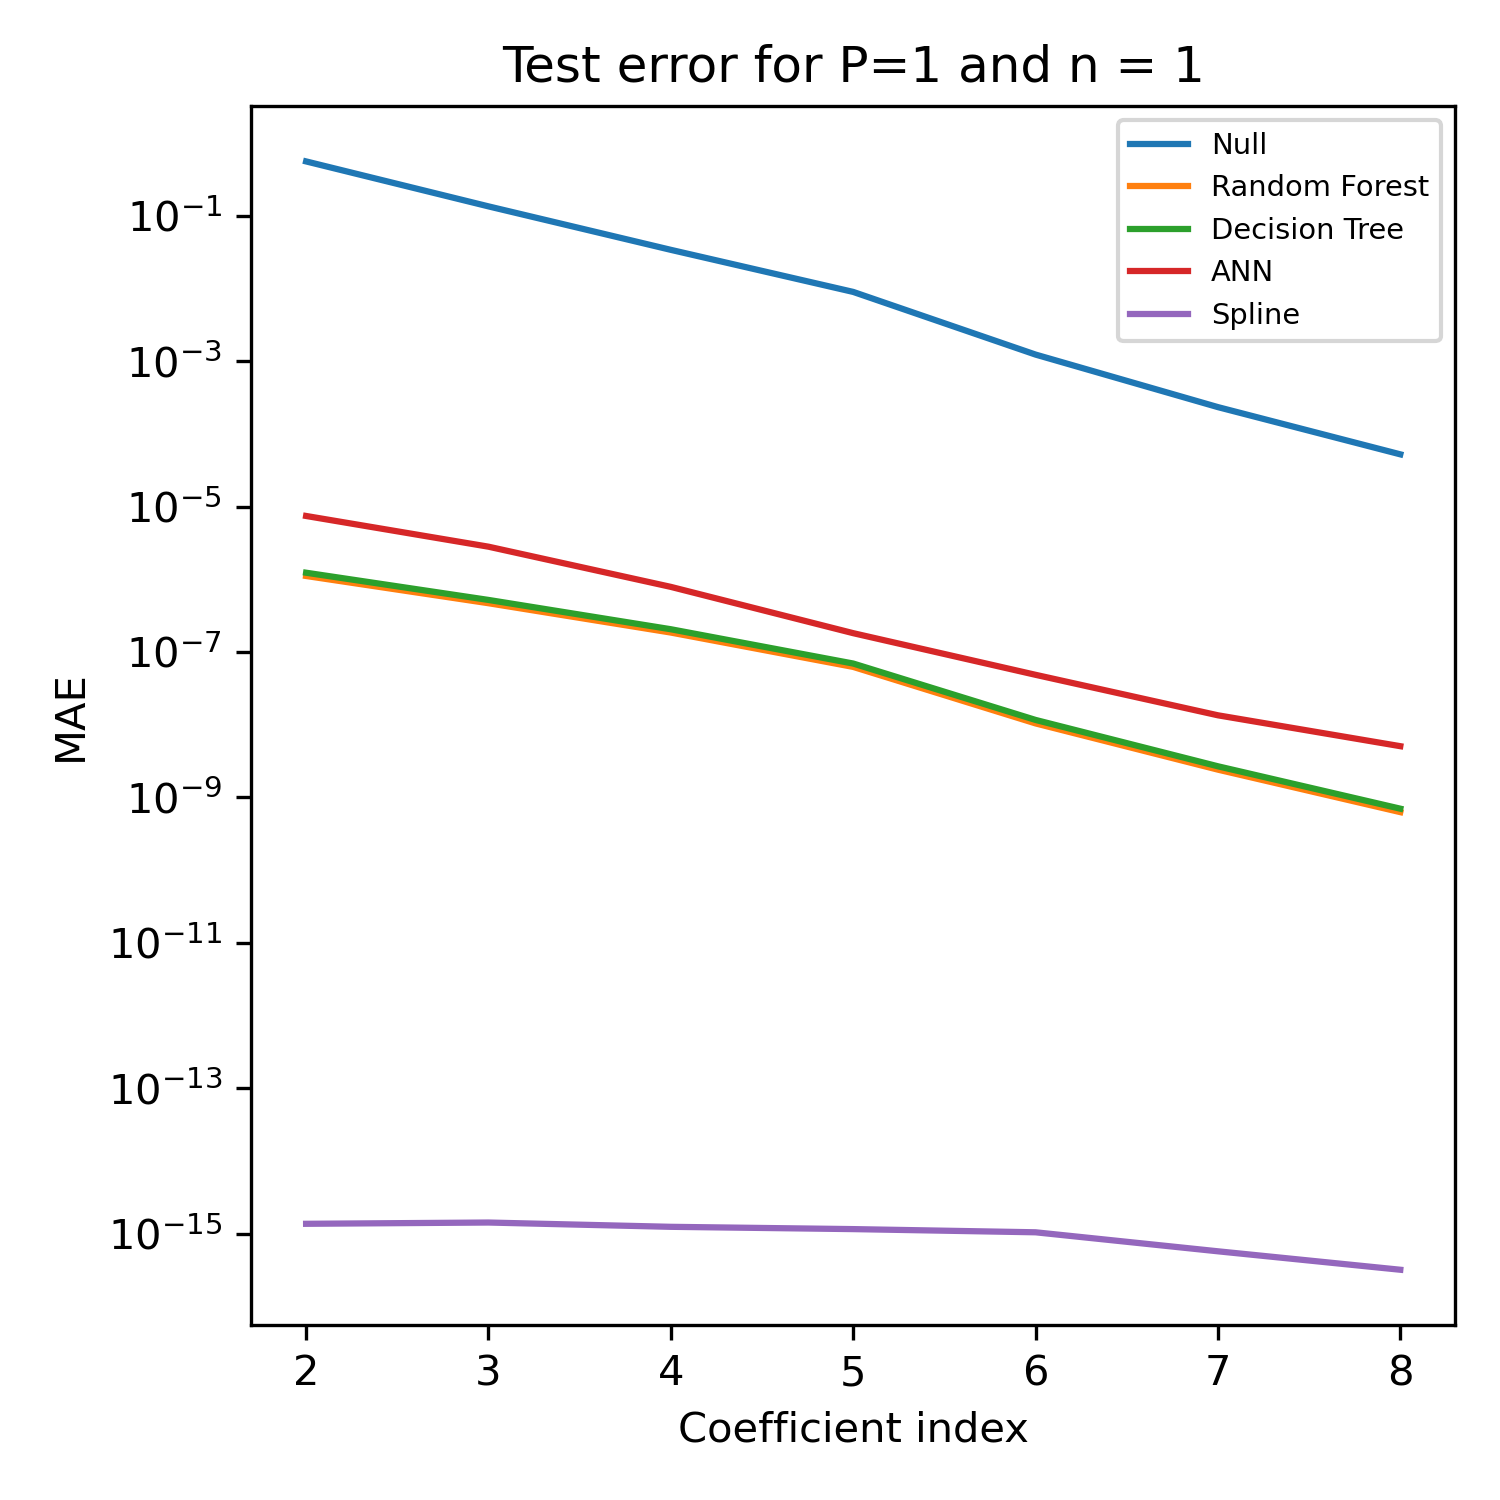
\includegraphics[width=\linewidth]{Images/MLP1n1.png}
                \end{minipage} &
                \begin{minipage}{0.16\textwidth}
                    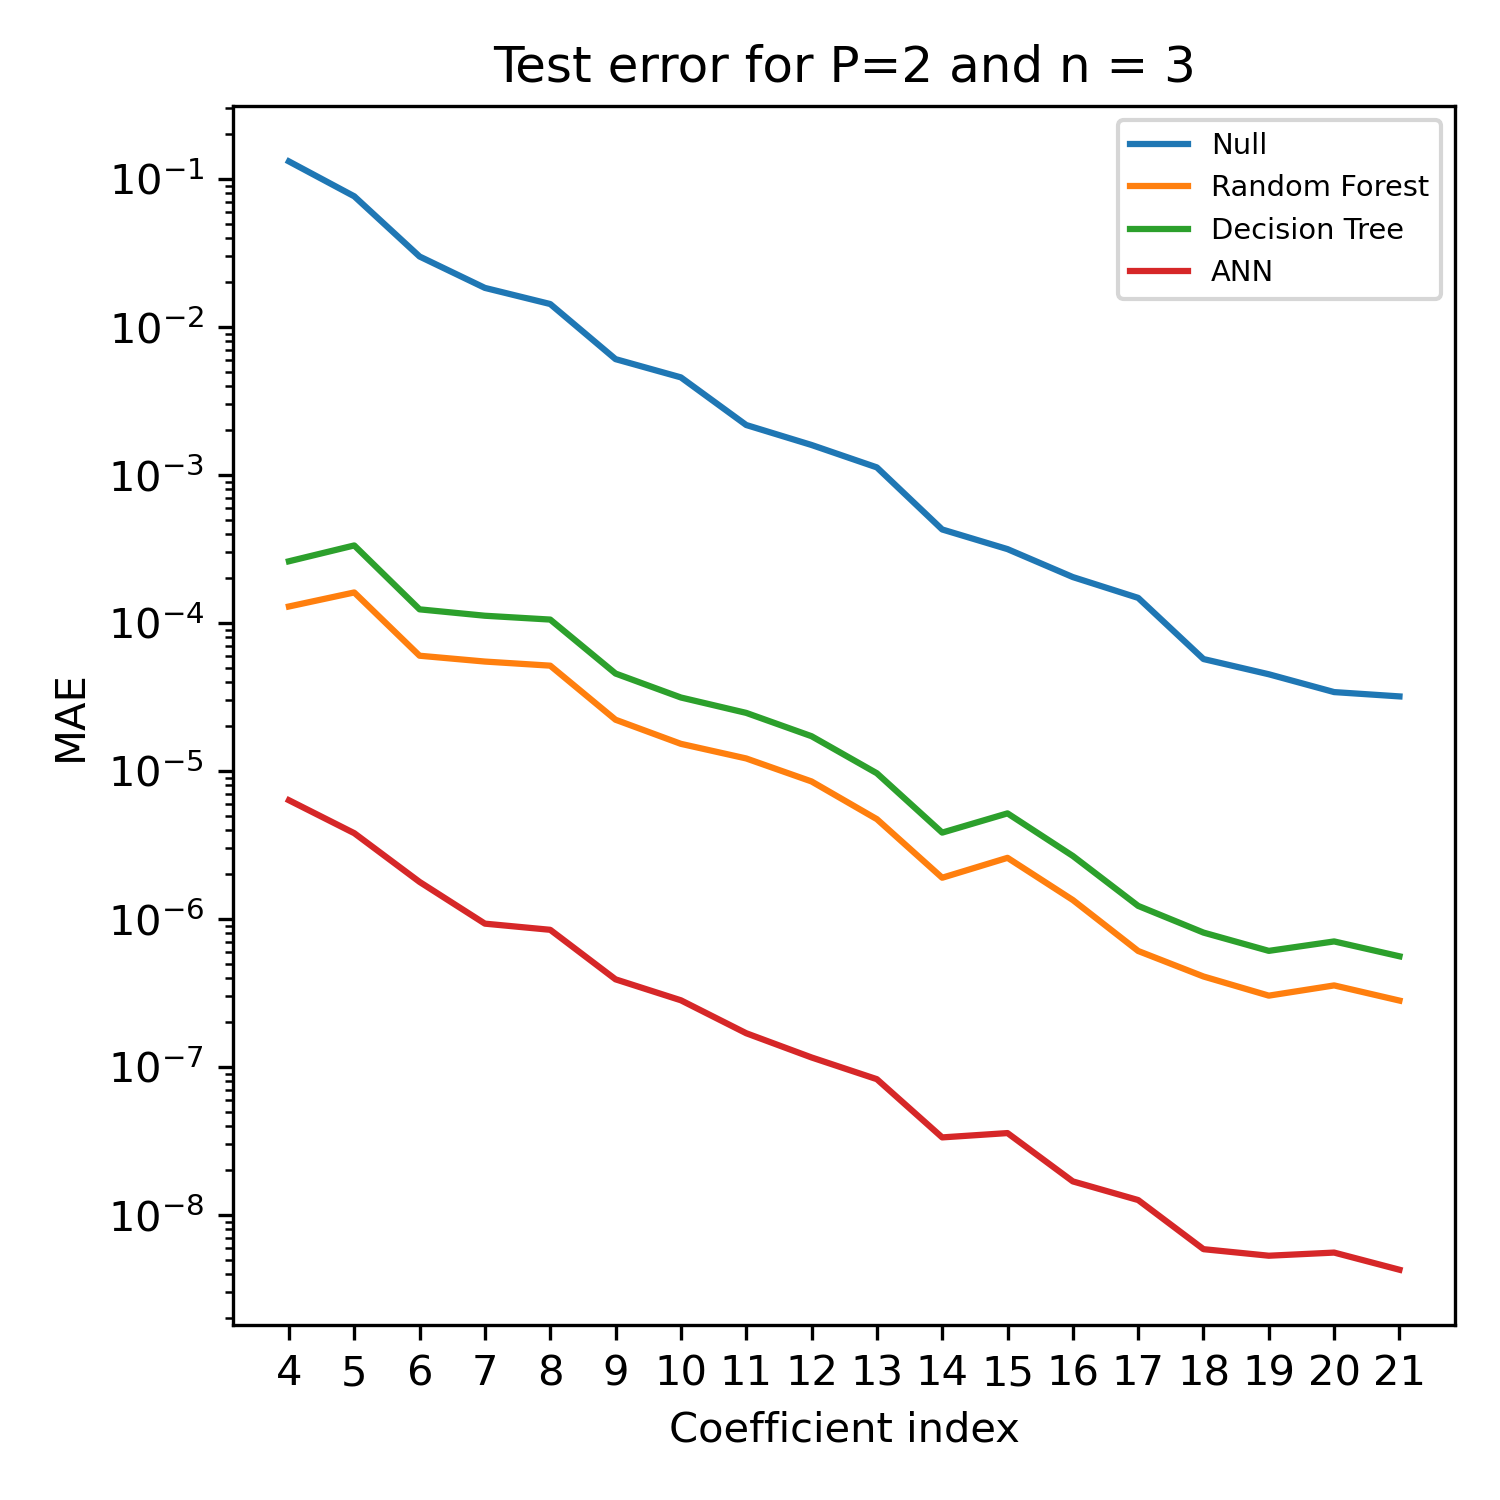
\includegraphics[width=\linewidth]{Images/MLP2n3.png}
                \end{minipage} \\
                \begin{minipage}{0.16\textwidth}
                    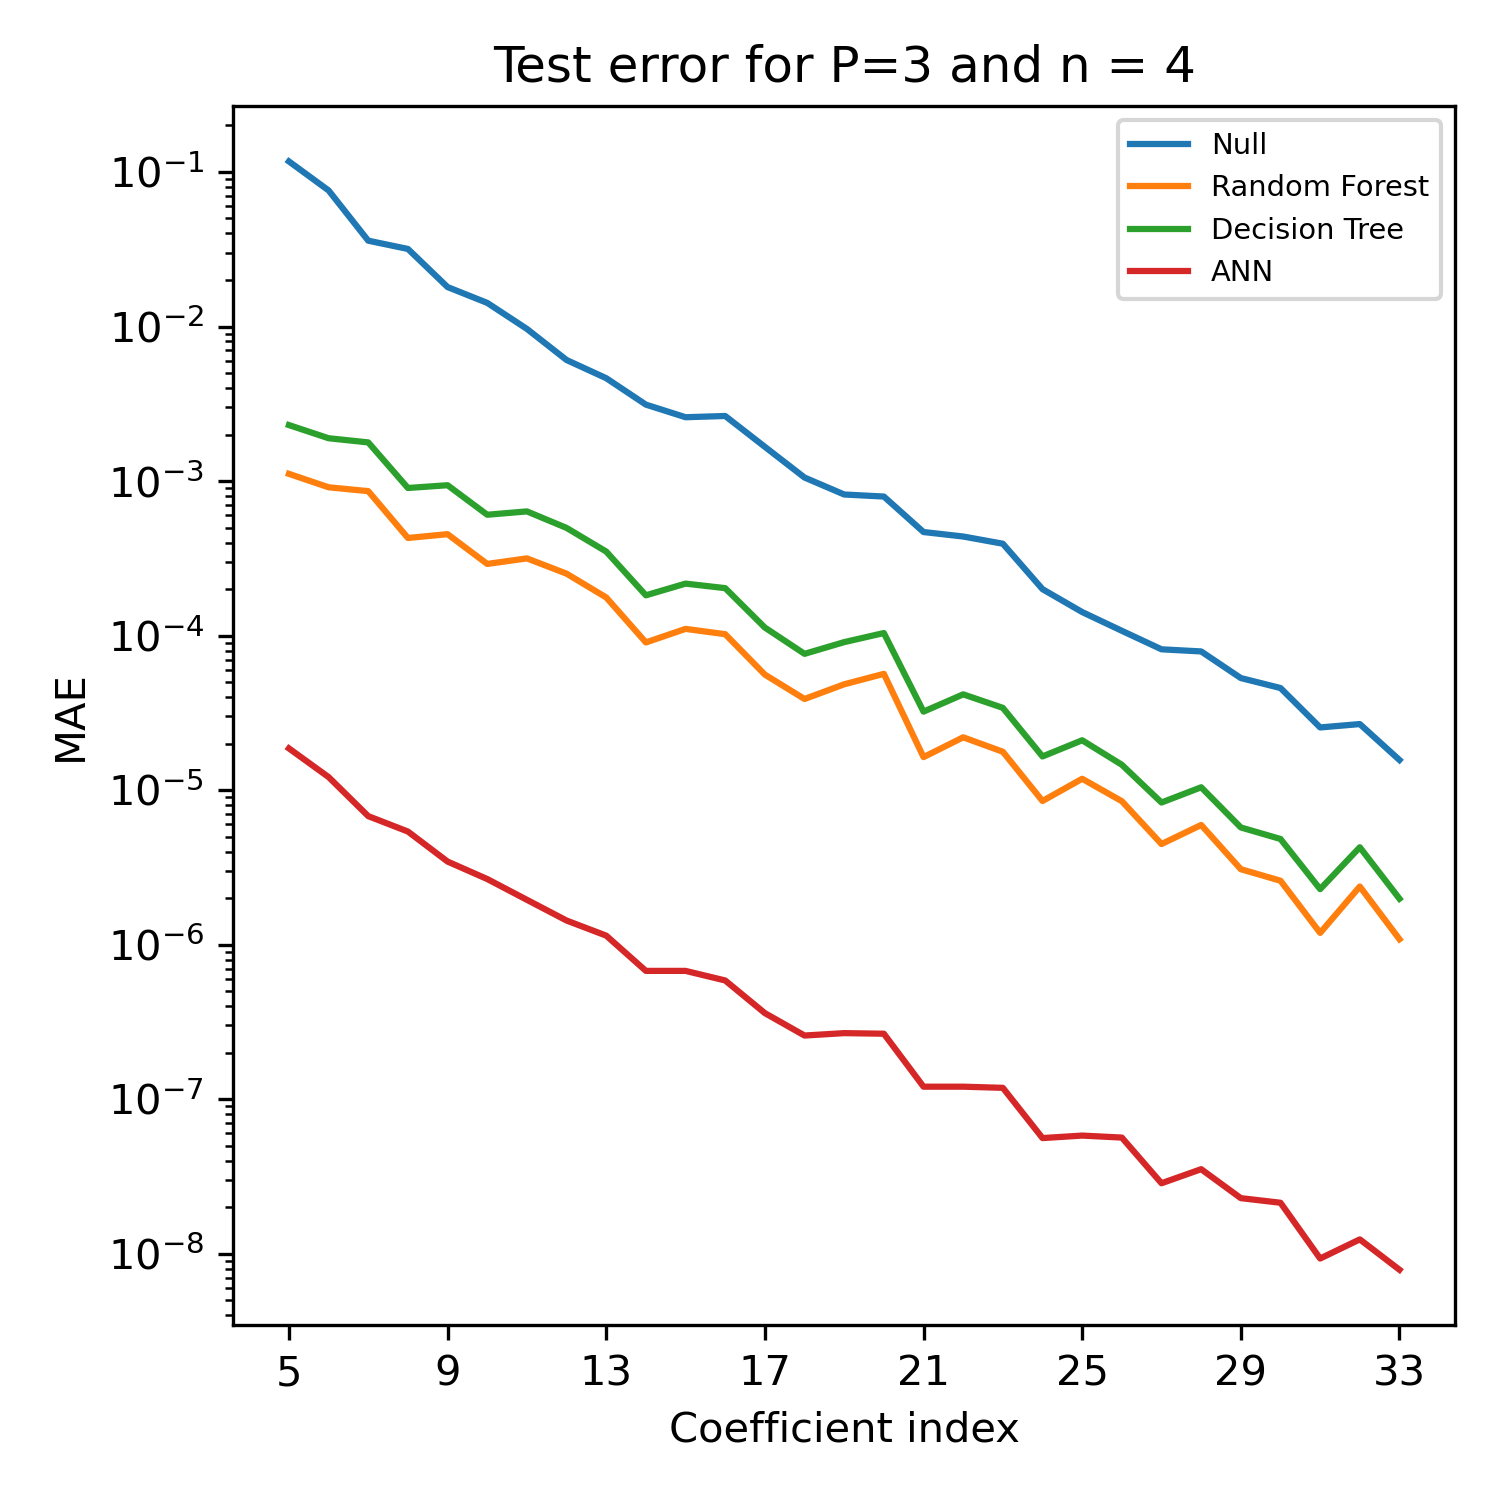
\includegraphics[width=\linewidth]{Images/MLP3n4.png}
                \end{minipage} &
                \begin{minipage}{0.16\textwidth}
                    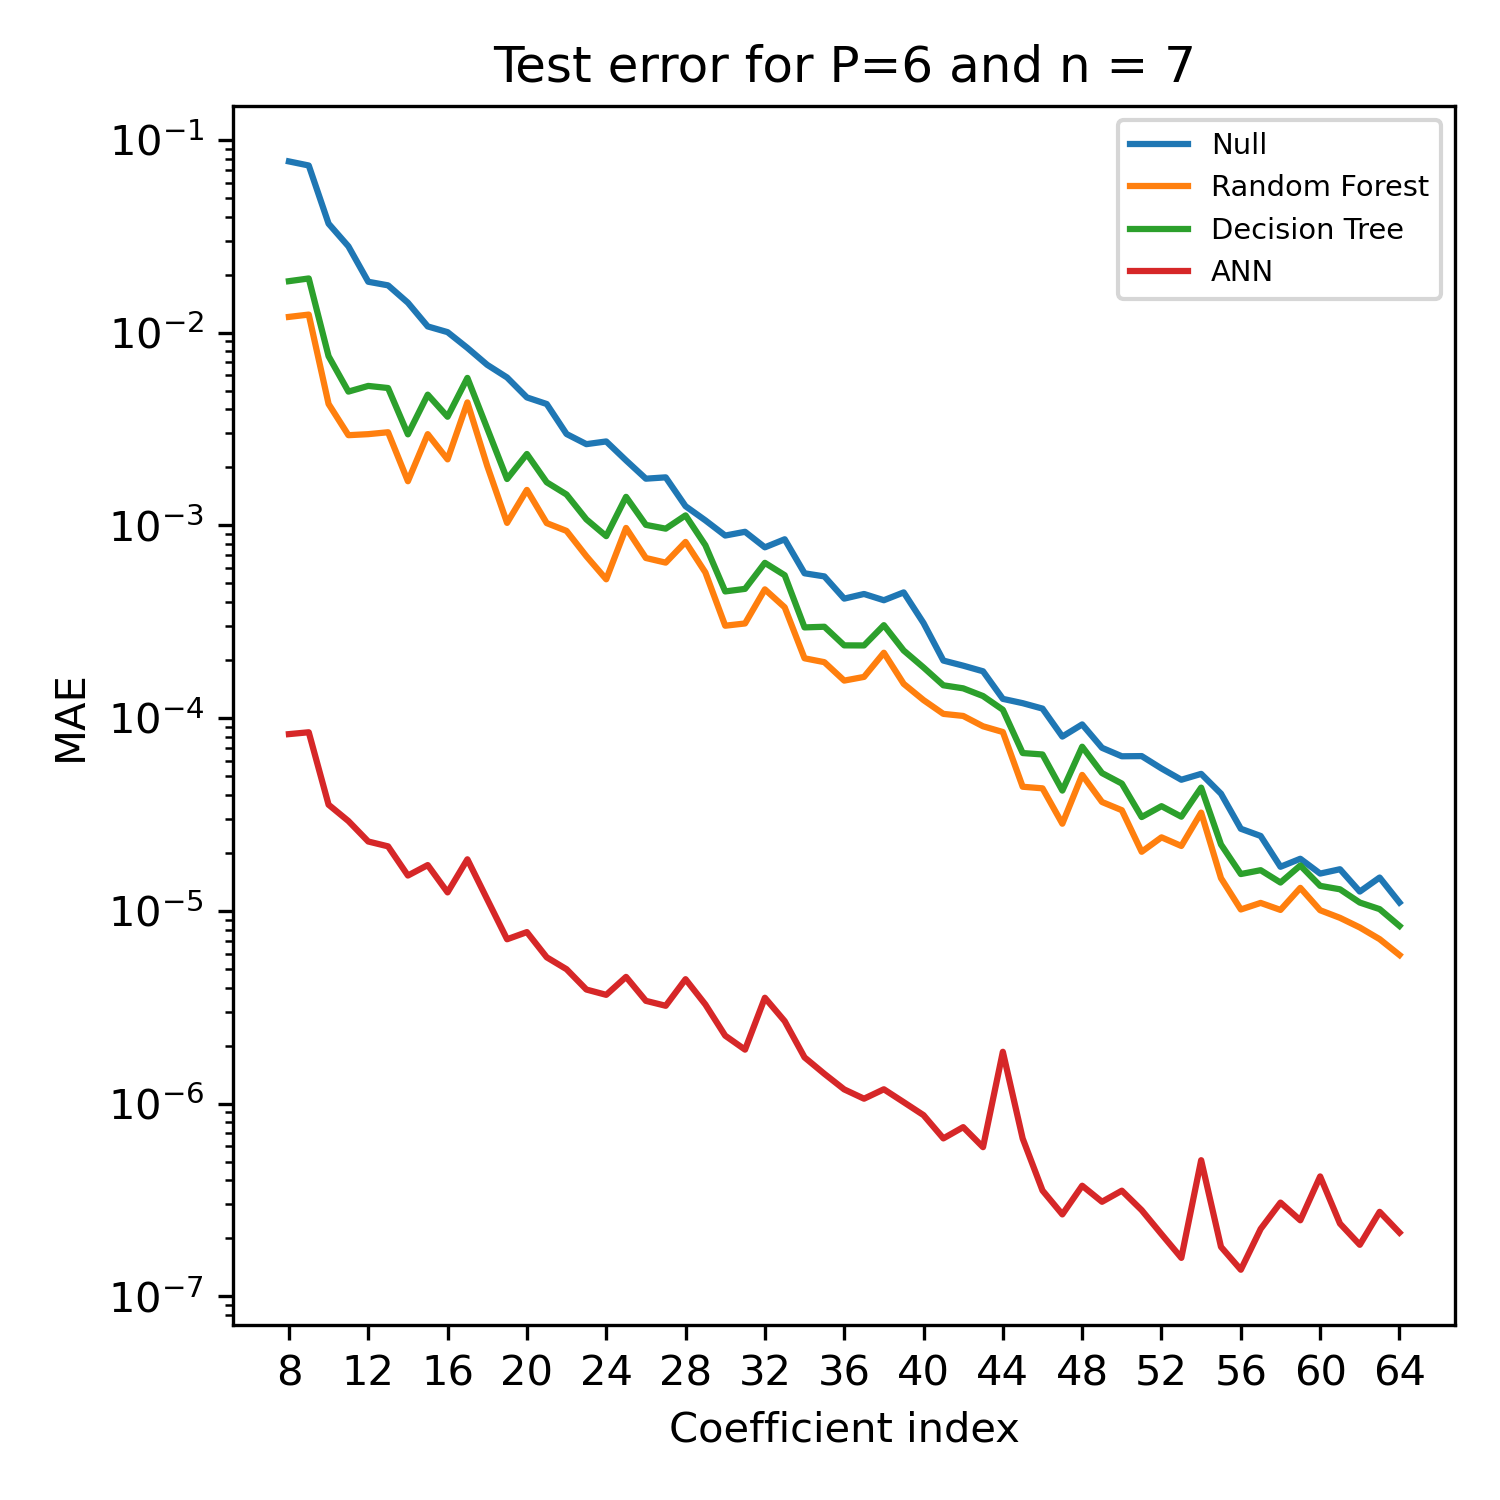
\includegraphics[width=\linewidth]{Images/MLP6n7.png}
                \end{minipage}
            \end{tabular}
        \end{center}

    }
    
    \block{\large Practical Notes}
    {
        \small
        \begin{itemize}
            \item Given an accurate regression model, NL-C RBM can achieve the same accuracy as the classical RBM with a dependence on significantly fewer modes (coefficients). Otherwise, the regression error becomes dominant.
            \item NL-C RBM would have a time advantage over the classical RBM when $N \gg n$ see \cite{BARNETT2023112420}, which is not the case in our current test case.
            \item The NL-C RBM Galerkin formulation in (\ref{eq:galerkin_Nl}) is not necessary well posed. A better approach would be to minimize the residual over the first $n$ coefficients.
            \item While ANNs have a higher inference cost than other models, they achieve superior accuracy in high-dimensional settings.
        \end{itemize}

    } 

} 

\column{0.55}{

    \block{\large On the choice of  \textbf{ n = P}}
    {        
        \small
        $$    
        \sum_{j=1}^N \alpha_j^r (\boldsymbol{\mu})  \varphi_{j}^r \overset{\textbf{SVD}}{\longleftarrow}   u(\boldsymbol{\mu}) - u(\boldsymbol{\mu_0}) \overset{\textbf{Taylor}}{\approx}   \sum_{j=1}^P (\mu^j-\mu_0^j) \frac{\partial u}{\partial \mu^j}(\boldsymbol{\mu_0})    \overset{\textbf{SVD}}{\longrightarrow}  \sum_{j=1}^P \alpha_j^* (\boldsymbol{\mu}) \varphi_{j}^*,\text{ for }\boldsymbol{\mu} \in {\mathcal B}(\boldsymbol{\mu_0}, r) \subset \mathbb{R}^{P}.
        $$
        
        \begin{itemize}
            \item $\boldsymbol{\mu} \mapsto \bigl(\alpha_j^* (\boldsymbol{\mu})\bigr)_{j=1,..,p}$ is linear and bijective.
            \item $||\phi_j^r - \phi_j^*||_{L^2} \underset{r \rightarrow 0}{\longrightarrow} 0, \, \,\forall j \in \{1,\dots,P\} \implies \exists R>0, \, \boldsymbol{\mu} \mapsto \bigl(\alpha_j^r (\boldsymbol{\mu})\bigr)_{j=1,..,p} $ is bijective for any $r\le R$.

        \end{itemize}
        \textbf{Conclusion:} All the information, close enough to $\boldsymbol{\mu_0}$ is present in the first $P$ coefficients. As a result, one can choose {\color{myDarkRed} \underline{\underline{$\boldsymbol{n=P}$}}} (resp {\color{myDarkRed} \underline{\underline{$\boldsymbol{n=P+1}$}}} if the manifold is not centered , i.e., without subtracting  $u(\boldsymbol{\mu_0})$) locally. Away from $\boldsymbol{\mu_0}$, this may not be true anymore, the information may be in other modes than the first $P$ ones  (resp $P+1$ ones), or we may need more modes than $P$ (resp $P+1$).

    }
    \block{\large Test case: the multiparameter problem}{
        \small
        We design a thermal fin to effectively remove heat from a surface. The fin is characterized by a parameter vector $\boldsymbol{\mu} = (k^1, \ldots, k^{N_{fins}}, Bi)$, where $k^i$ is the thermal conductivity of the $i$-th subfin and $Bi$ is the Biot number. The variational formulation of the problem is given by: find $u(\boldsymbol{\mu}) \in X$ s.t

        \begin{tabular}{cc}
            \begin{minipage}{0.3\textwidth}
                \vspace{-1cm}
                \begin{equation*}
                    \footnotesize
                    \overbrace{\sum_{i=0}^{N_{fins}} \int_{\Omega_i} k^i \nabla u(\boldsymbol{\mu}) \cdot \nabla v \, dx + Bi  \int_{\Gamma_{ext}} u(\boldsymbol{\mu}) \, v \, dx}^{a(u(\boldsymbol{\mu}),v;\boldsymbol{\mu})} = \overbrace{\int_{\Gamma_{root}} v \, dx}^{\ell(v)} \quad \forall v \in X
                \end{equation*}
            \end{minipage}  &
            \hspace{-10cm}
            \begin{minipage}{0.5\textwidth}
                \centering
                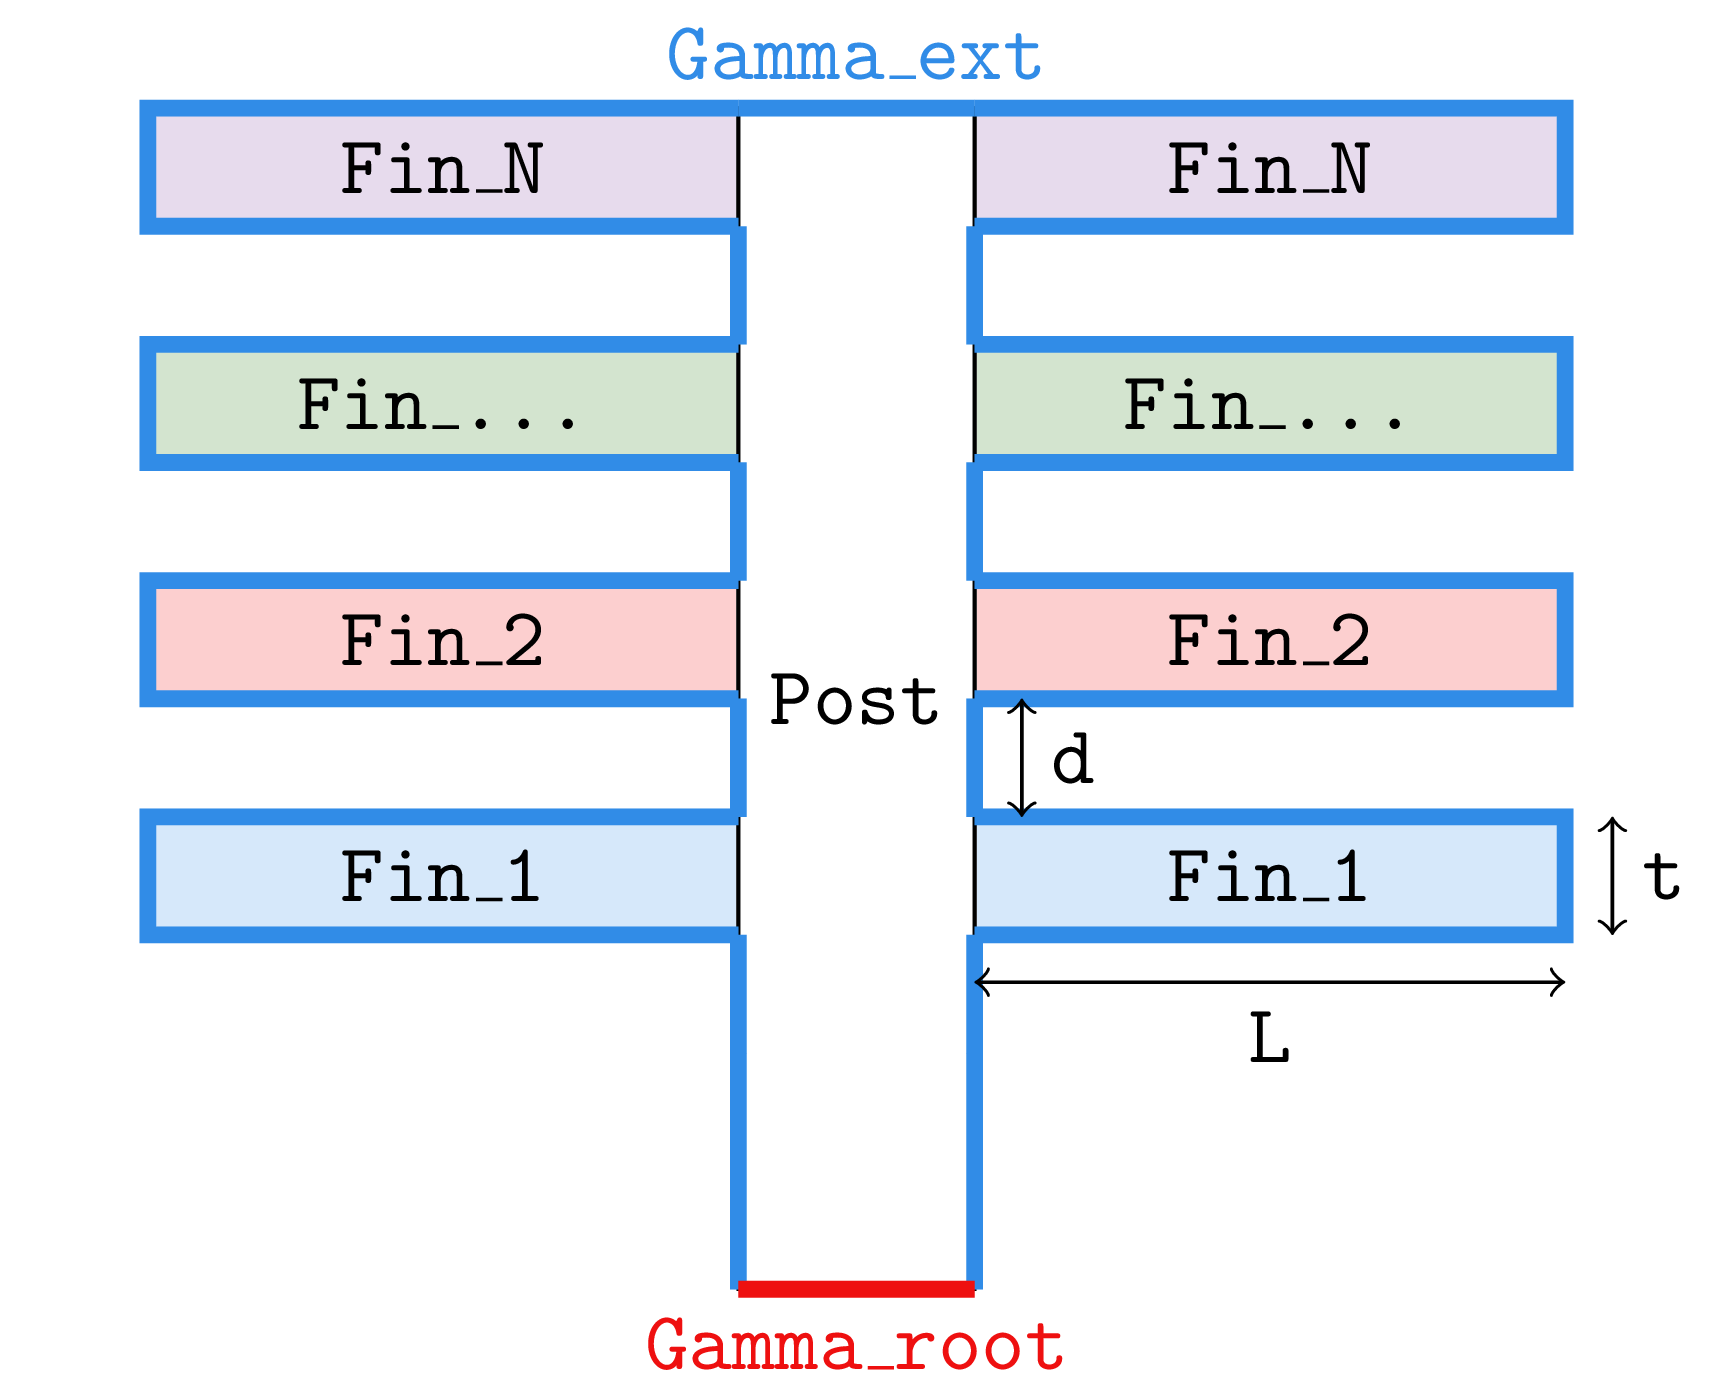
\includegraphics[width=0.18\textwidth]{Images/thermal-fin.png}
            \end{minipage}
        \end{tabular}


 

        In this work, we set $N_{fins} = 5$ so we can increase the parameter dimension up to $P=6$. The FOM is obtained by a second-order finite element space of dimension $N_h = 89745$. All the computations are performed using \textbf{Feel++} library.
    } % end of block

    \block{\large Nonlinear compressive RBM in action}
    {
        \small
                \textbf{Galerkin approach:} Find $u_{n}(\boldsymbol{\mu}) \in X_n=\text{span}\{\varphi_1, \ldots, \varphi_n\}$ s.t
                \begin{equation}
                    \label{eq:galerkin_Nl}
                    a(u_{n}(\boldsymbol{\mu}),v;\boldsymbol{\mu}) + a(\sum_{k=n+1}^{N} \psi^k(u_{n}(\boldsymbol{\mu})) \, \varphi_k,v;\boldsymbol{\mu}) = \ell(v) \quad \forall v \in X_n
                \end{equation}

                \textbf{P=1 (scalar parameter) and n=1}:\vspace{0.5cm}

                    \begin{tabular}{|l|c|c|c|}
                        \hline
                        \textbf{Model} & \textbf{Mean Energy Error} & \textbf{Mean L2 Error} & \textbf{Max L2 Error}\\
                        \hline
                        RB (with 8 modes) & $1.01 \times 10^{-5}$ & $5.89 \times 10^{-6}$ & $1.74 \times 10^{-5}$  \\
                        \hline
                        RB (with 1 mode) & $5.52 \times 10^{-1}$ & $6.57 \times 10^{-1}$ & $2.49 \times 10^{0}$ \\
                        \hline
                        Random Forest & $1.05 \times 10^{-5}$ & $9.82 \times 10^{-6}$ & $7.23 \times 10^{-5}$ \\
                        \hline
                        Spline & $1.01 \times 10^{-5}$ & $5.89 \times 10^{-6}$ & $1.74 \times 10^{-5}$ \\
                        \hline
                        ANN & $1.41 \times 10^{-5}$ & $1.13 \times 10^{-5}$ & $3.87 \times 10^{-5}$ \\
                        \hline
                    \end{tabular}
                
            
                \begin{tikzpicture}[overlay]
                    % Arrow from RB (with 8 modes)
                    \draw[->, myDarkRed, line width=2mm] (23.5,4) -- ++(1,-1) node[right, align=left, black] {We achieve the\\ same accuracy.};
                    % Arrow from Spline
                    \draw[->, myDarkRed, thin, line width=2mm] (23.5,1.5) -- ++(1,1);
                \end{tikzpicture}

                \vspace{1cm}
                \textbf{P=2 (2D parameter space) and n=3:}\vspace{0.5cm}

                \begin{tabular}{|l|c|c|c|}
                    \hline
                    \textbf{Model} & \textbf{Mean Energy Error} & \textbf{Mean L2 Error} & \textbf{Max L2 Error} \\
                    \hline
                    RB (with 21 modes) & $2.19 \times 10^{-5}$ & $1.30 \times 10^{-5}$ & $2.54 \times 10^{-5}$ \\
                    \hline
                    RB (with 3 modes) & $1.66 \times 10^{-1}$ & $1.52 \times 10^{-1}$ & $5.23 \times 10^{-1}$ \\
                    \hline
                    Random Forest & $2.93 \times 10^{-4}$ & $1.89 \times 10^{-4}$ & $7.04 \times 10^{-4}$  \\
                    \hline
                    ANN & $2.41 \times 10^{-5}$ & $1.43 \times 10^{-5}$ & $2.80 \times 10^{-5}$ \\
                    \hline
                \end{tabular}      
          

                \vspace{1cm}
                \textbf{P=3 (3D parameter space):}\vspace{0.5cm}

                \begin{tabular}{|l|c|c|c|}
                    \hline
                    \textbf{Model} & \textbf{Mean Energy Error} & \textbf{Mean L2 Error} & \textbf{Max L2 Error}  \\
                    \hline
                    RB (with 33 modes) & $2.06 \times 10^{-5}$ & $7.43 \times 10^{-6}$ & $1.88 \times 10^{-5}$ \\
                    \hline
                    RB (with 4 modes) & $1.92 \times 10^{-1}$ & $2.49 \times 10^{-1}$ & $9.05 \times 10^{-1}$ \\
                    \hline
                    Random Forest & $3.43 \times 10^{-3}$ & $4.14 \times 10^{-3}$ & $2.59 \times 10^{-2}$ \\
                    \hline
                    ANN & $3.56 \times 10^{-5}$ & $2.60 \times 10^{-5}$ & $6.98 \times 10^{-5}$ \\
                    \hline
                \end{tabular}

                \vspace{1cm}
                                
    }



    \block{\large References}
    {
        \nocite{*}
        \printbibliography[heading=none]

        \vspace{0.5cm}
        \small
        \textbf{Acknowledgment:} 	As part of the “France 2030” initiative, this work has benefited from a national grant managed by the French National Research Agency (Agence Nationale de la Recherche), attributed to the ExaMA project of the NumPEx PEPR program under reference ANR-22-EXNU-0002, and has also been funded in part by the European Research Council (ERC) under the European Union’s Horizon 2020 research and innovation program (grant No. 810367), project EMC2 (Y.M.).
    

    } 

     

  

}

\end{columns}

\end{document}